% 
% MANUAL DOCUMENT 
% ===============
% 
% Time-stamp: <2010-03-23 16:27:45>
% (c) 2009 The JAGSAT development team.
% 

\documentclass[12pt,a4paper]{article}

\usepackage{raskolnikov}

\title{\large JAGSAT project\\\huge Game manual}
\author{
  Juan Pedro Bolívar Puente\\ 
  Aksel Junkkila\\
  Guillem Medina\\ 
  Sarah Lindstrom\\ 
  Alberto Villegas Erce\\ 
  Thomas Forss
}
\location{Project Course \\ \textit{Åbo Akademy}}
% \date{}

%\disabletodo 

\begin{document}

\maketitle

\begin{center}
\textbf{Revision history}

\begin{tabular}{ l | l | l | l }
Date			&Version	&Description		&Author\\\hline\hline
22.03.2009	&1.0		&Creation			&Alberto Villegas 
\end{tabular}
\label{tab:rev}
\end{center}

\vfill
Copyright 2009 AUTHORS.
Permission is granted to copy, distribute and/or modify this document under the terms of the GNU Free Documentation License, Version 1.1 or any later version published by the Free Software Foundation;  with no Invariant Sections, with no Front-Cover Texts, and with no Back-Cover Texts. A copy of the license is included in the ``D9: Licenses''  document entitled `GNU Free Documentation License''.

\pagebreak
\tableofcontents
\pagebreak

\section{Introduction}
Welcome to the "Code of Greed" manual. In this classic "Global Domination" game  you are battling to conquer the world. To win, you must launch daring attacks, defend yourself on all fronts, and sweep across vast continents with boldness and cunning. But remember, the dangers, as well as the rewards, are high. Just when the world is within your grasp, your opponent might strike and take it all away.

\section{Object of the game}
The object of the game is to be the first player to complete the Mission described on your own mission section.

\section{Equipment}
The following subsections describe the virtual elements that compose the game. You will interact with them all along the gameplay.

\subsection{World map}
The world map is made up of continents and each continent of a number of regions. There will be regions you own, where you will be able to place and move troops, and others that your enemies own, which you will be able to attack and conquer.

The regions will be equally divided through the players at the beginning of the game and automatically placing one troop from the respective owner player in each region. Each region has a troop counter, of the color of the owner player, that shows how many troops there are in the region at that moment.

\begin{figure}[h!]
\centering
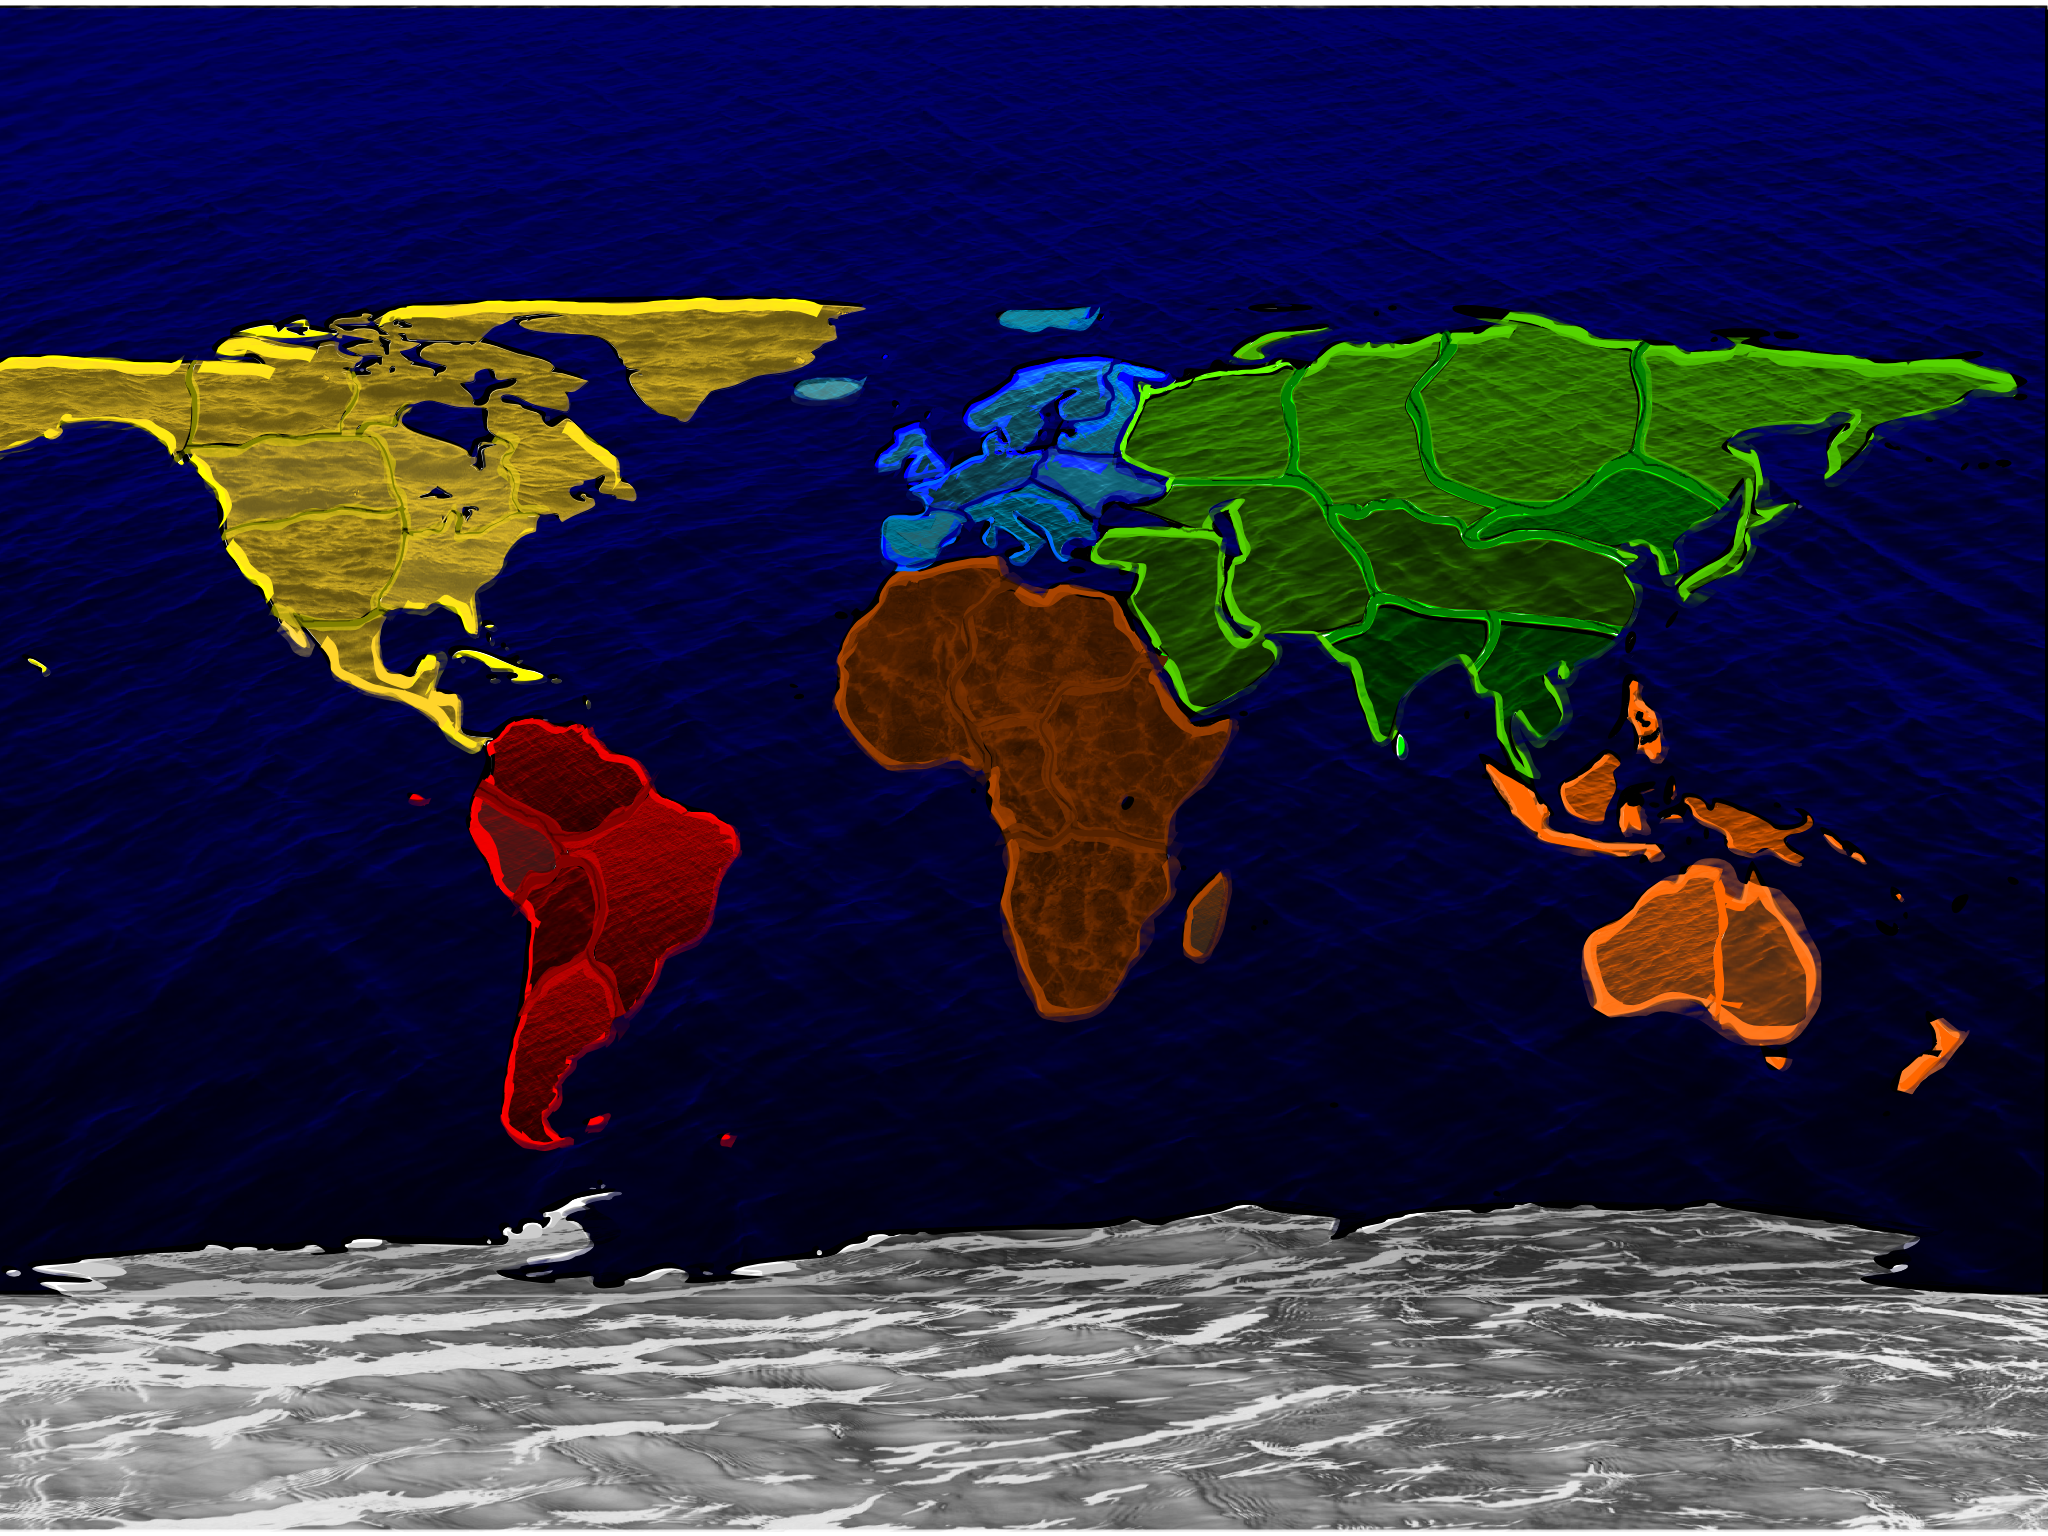
\includegraphics[width=6.5cm]{pic/map01.png}
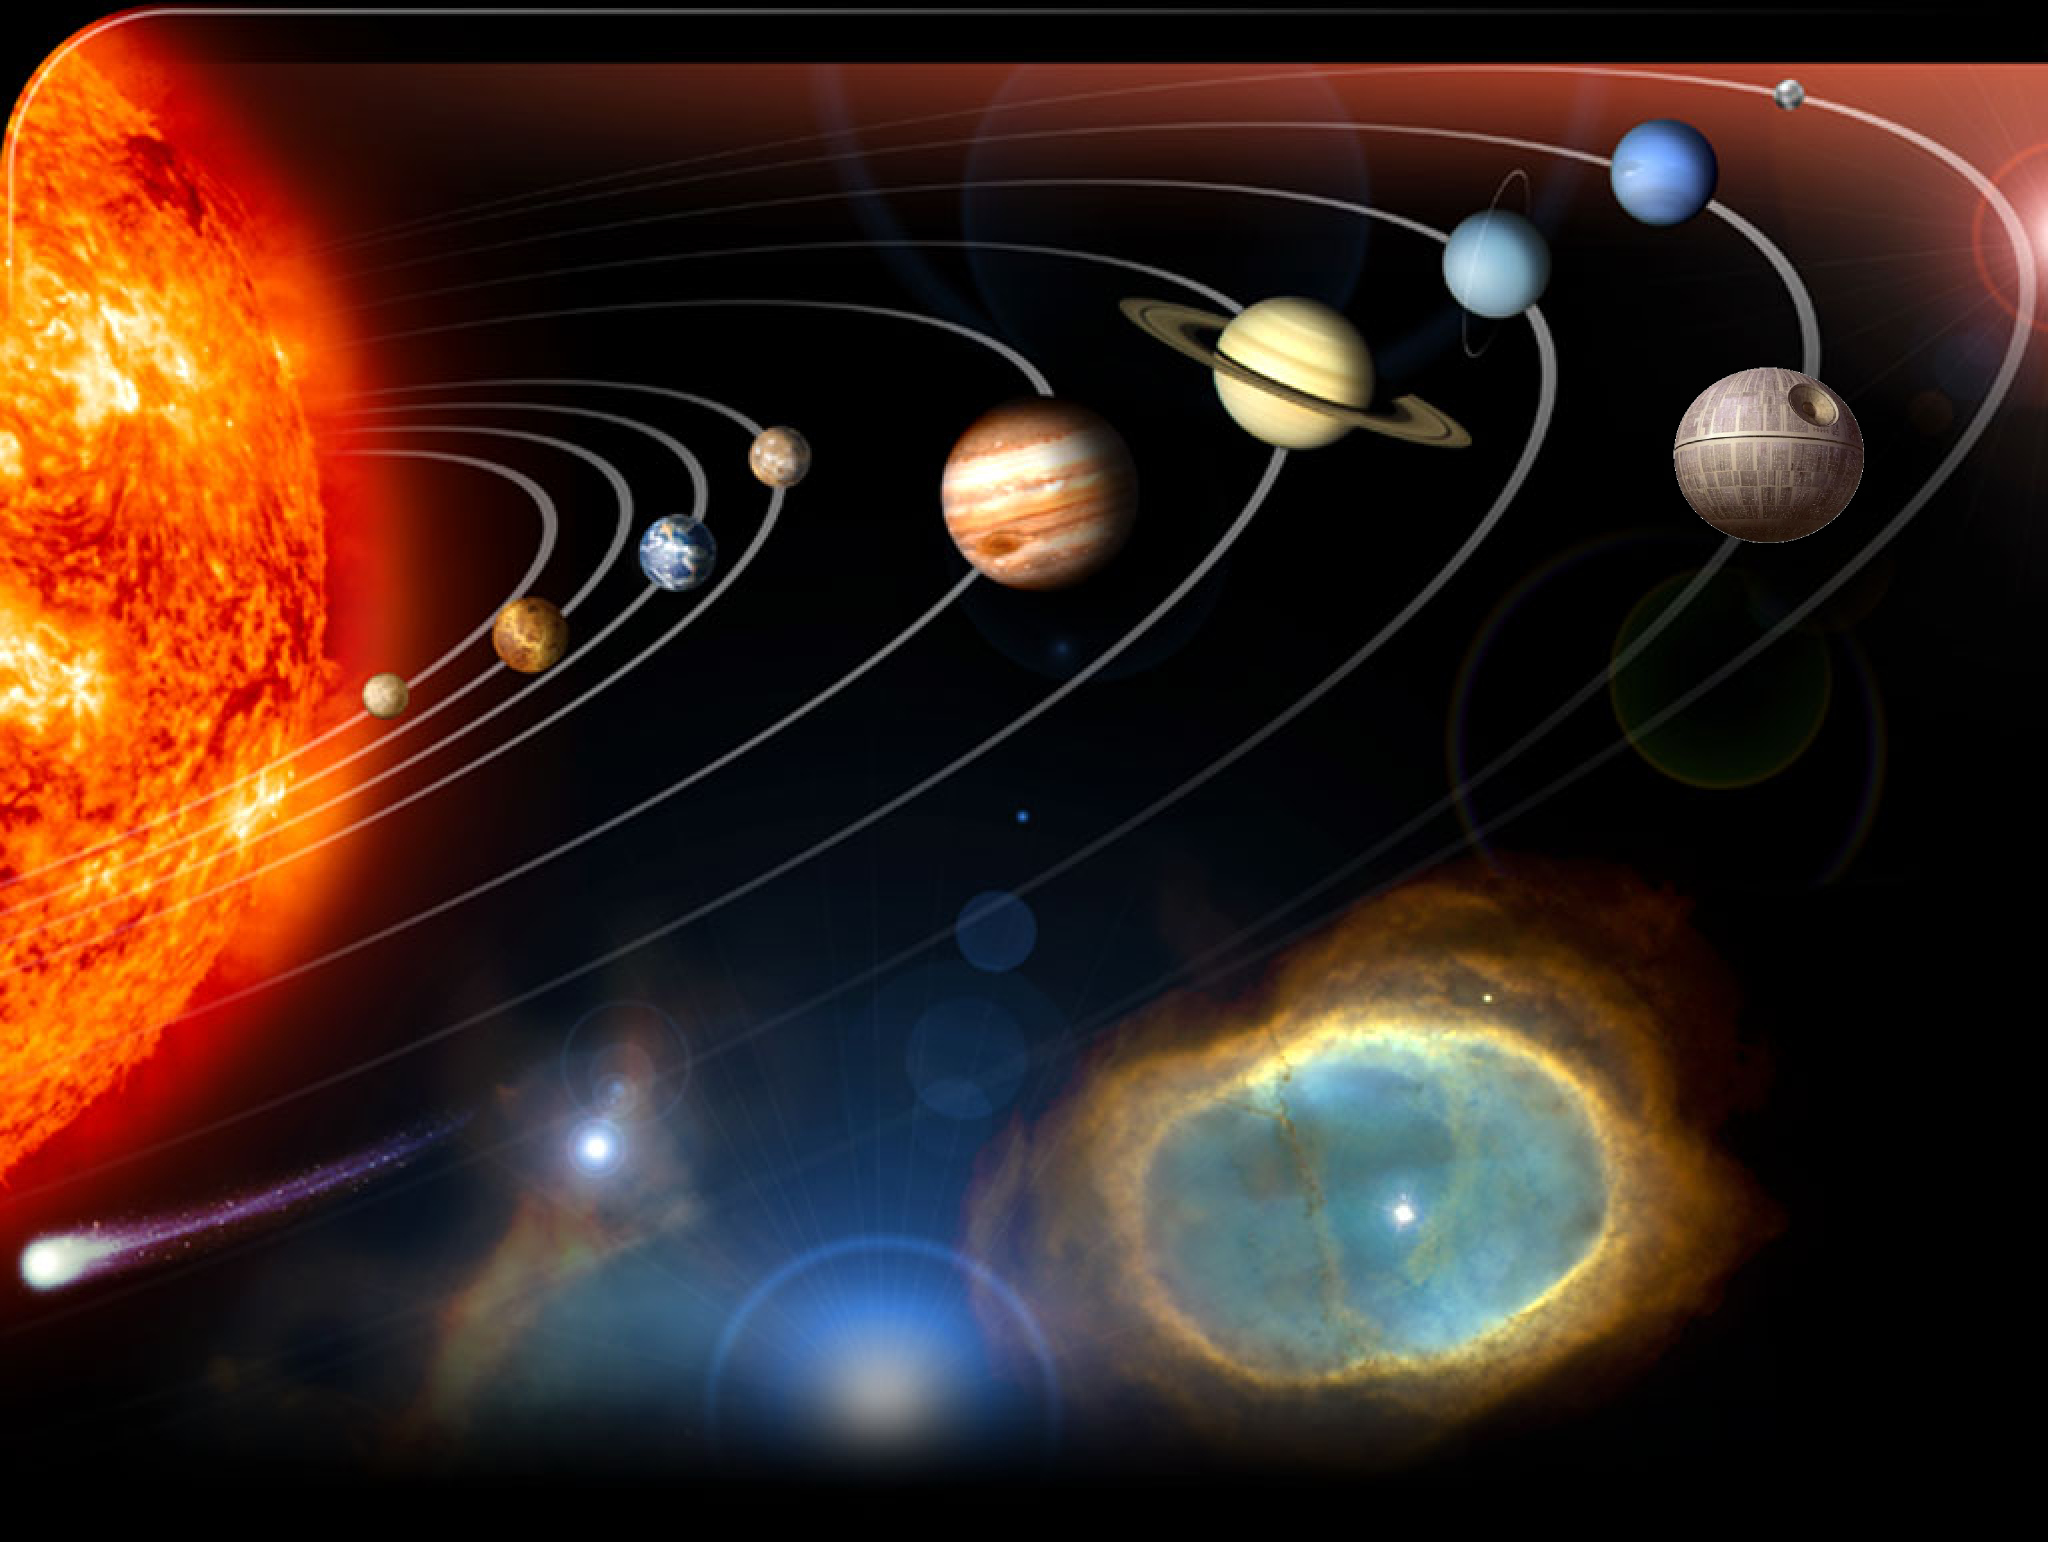
\includegraphics[width=6.5cm]{pic/map02.png}
\caption{Different world maps.}
\label{fig:map}
\end{figure}

\subsection{Troops}
Your troops are the basic elements that you will use to accomplish your mission. Your troops will be in your owned regions and will be the elements you will use to attack and conquer other regions. You need to have at least one troop per region in order to say that the region is yours.

\subsection{Cards}
Cards can be earned and trade all along the game play. They will be used in the reinforcement phase as an useful supplement of troops.

There are four kind of cards:

\begin{itemize}
\item {\bf Troop card}: represented with a {\it soldier}
\item {\bf Cavalry card}: represented with a {\it horse}
\item {\bf Cannon card}: represented with a {\it cannon}
\item {\bf Wild card}: represented with a {\it question mark}
\end{itemize}

\subsubsection{Earning cards}
At the end of any turn in which you have capture {\bf at least one} territory, you will automatically earn {\bf one} card. You can have a maximum of...

\begin{todo}[Alberto]
  This is not clear yet.
\end{todo}

\subsubsection{Trading cards for armies}
At the beginning of subsequent turns, in the reinforcement phase, you may trade in matched sets of cards and take additional armies in the following way:
 
\begin{itemize}
\item 3 troop cards combination:
\item 3 cavalry cards combination:
\item 3 cannon cards combination:
\item One of each combination:
\end{itemize}

\begin{todo}[Alberto]
  Ask JP about this
\end{todo}

\subsection{Mission}
At the beginning of the game every player will receive a secret mission. To win the game a player has to be the first accomplishing his mission. If the mission is accomplished at the end of the player turn the game will end automatically.

There are three kind of missions that are generated automatically based on the current world map: region type mission, continent type mission and player type mission.

\subsubsection{Region type mission}
Region type missions consist on conquering an indicated number of regions under certain circumstances.

The missions of this type are:

\begin{itemize}
\item Conquer 57\% of the total number of regions with at least one troop on each.
\item Conquer 43\% of the total number of regions with at least two troops on each.
\end{itemize}

\subsubsection{Continent type mission}
Continent type missions consist on conquering an indicated list of two or three continents.

\subsubsection{Player type mission}
Player type missions consist on defeating one enemy player. If you are the player that the mission orders to defeat or if the player has been killed by another player, the mission will automatically change to a region type mission.

\begin{todo}[Alberto]
  Is there any other "equipment" thing that should be explained?
\end{todo}

\section{Setup}
The game will start by setting everything up. Regions will be distributed and mission cards will be dealt automatically.

\begin{figure}[h!]
\centering
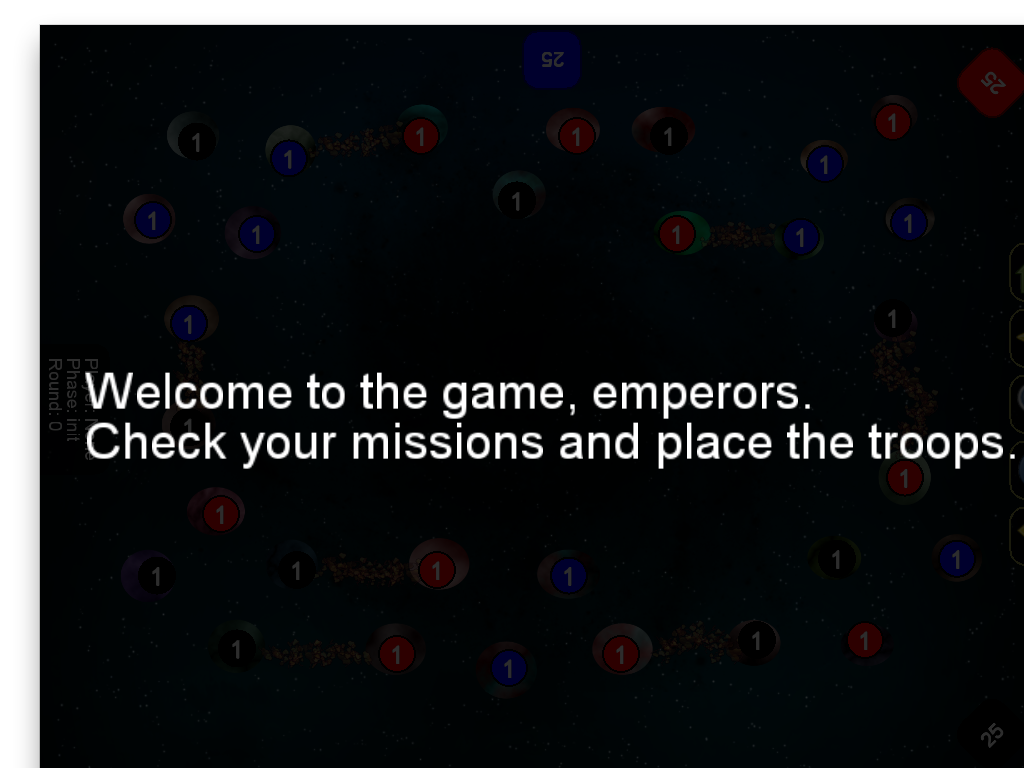
\includegraphics[width=10cm]{pic/screenshot01.png}
\caption{Introduction.}
\label{fig:setup}
\end{figure}

\subsection{Initial army placement}
Every player will have a number of remaining non-placed troops that he will have to place in his owned regions. Troops will be placed by clicking in the region counter. 

When all troops have been placed the first round will start automatically selecting a random initial player.

\begin{figure}[h!]
\centering
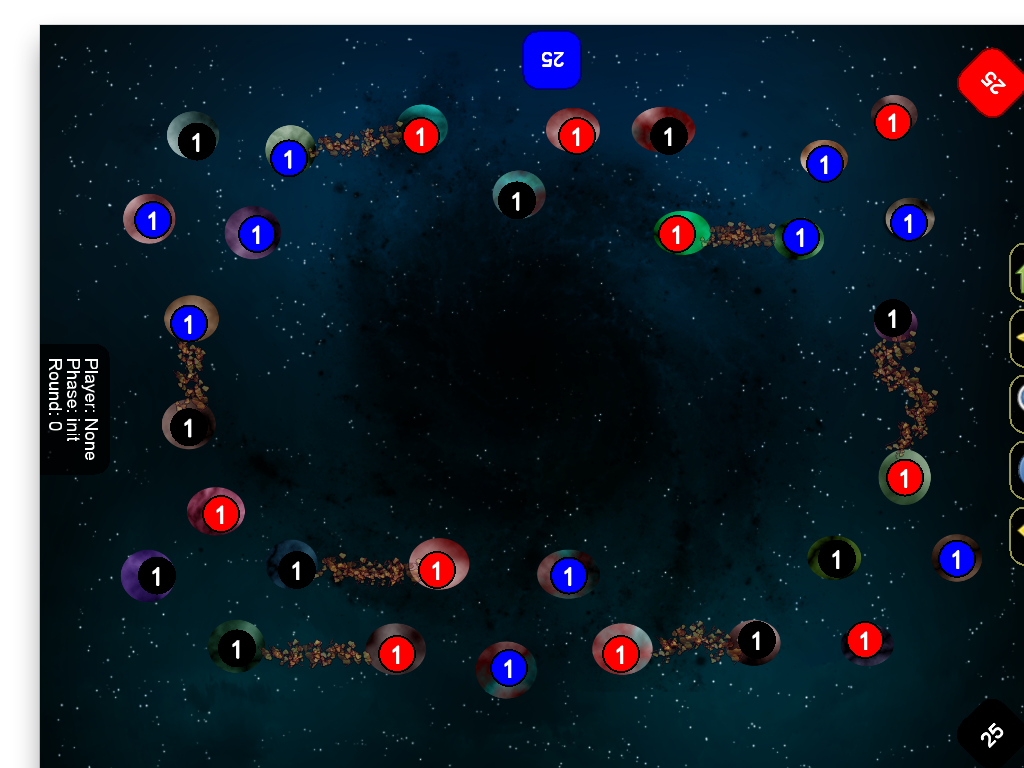
\includegraphics[width=10cm]{pic/screenshot02.png}
\caption{Region distribution.}
\label{fig:dist}
\end{figure}

\section{Playing}
The game rounds consist on three different phases: reinforcement, attack and movement. When a player finnish his round, right after the movement phase, the game will check if his mission has been attained. If it was so, the game will end, if it was not, next player (clockwise chosen) round will start.

\subsection{Reinforcement phase}
At the beginning of reinforcement phase you will receive a number of troops that will be calculated according with one or more of the following parameters:

\begin{itemize}
\item Number of territories you own: you will receive one troop for each 3 regions you own. 
\item Value of continents you control: each continent has an especial value.
\item The cards you use: you will get additional troops for them.
\end{itemize}

\begin{figure}[h!]
\centering
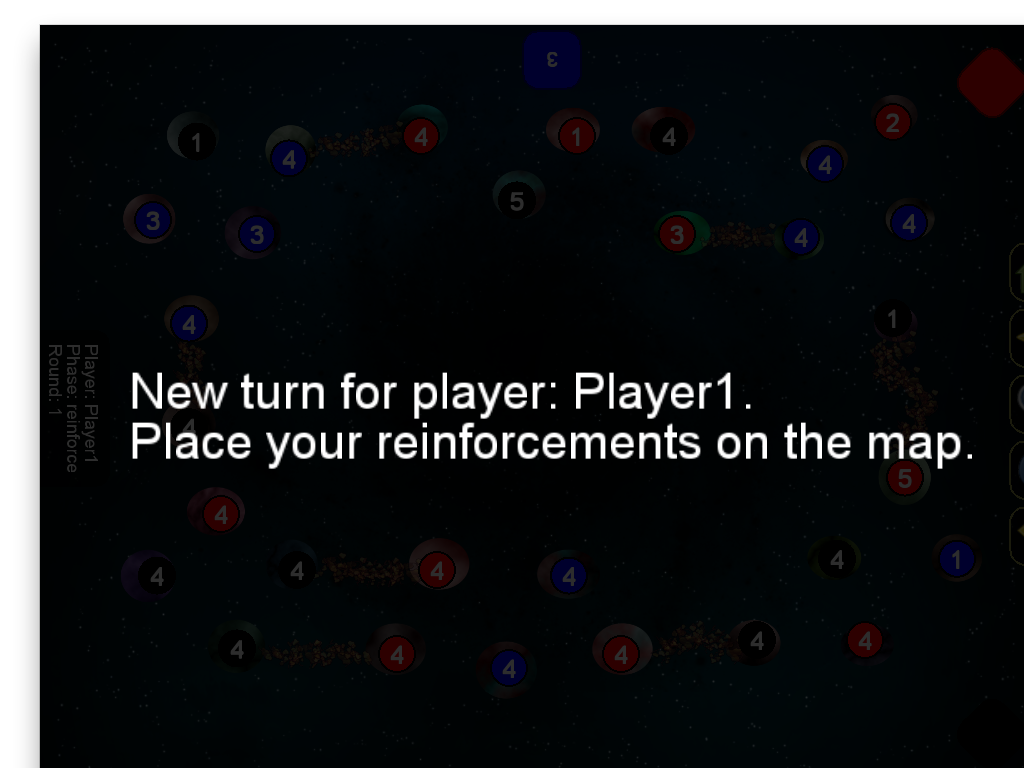
\includegraphics[width=6.5cm]{pic/screenshot03.png}
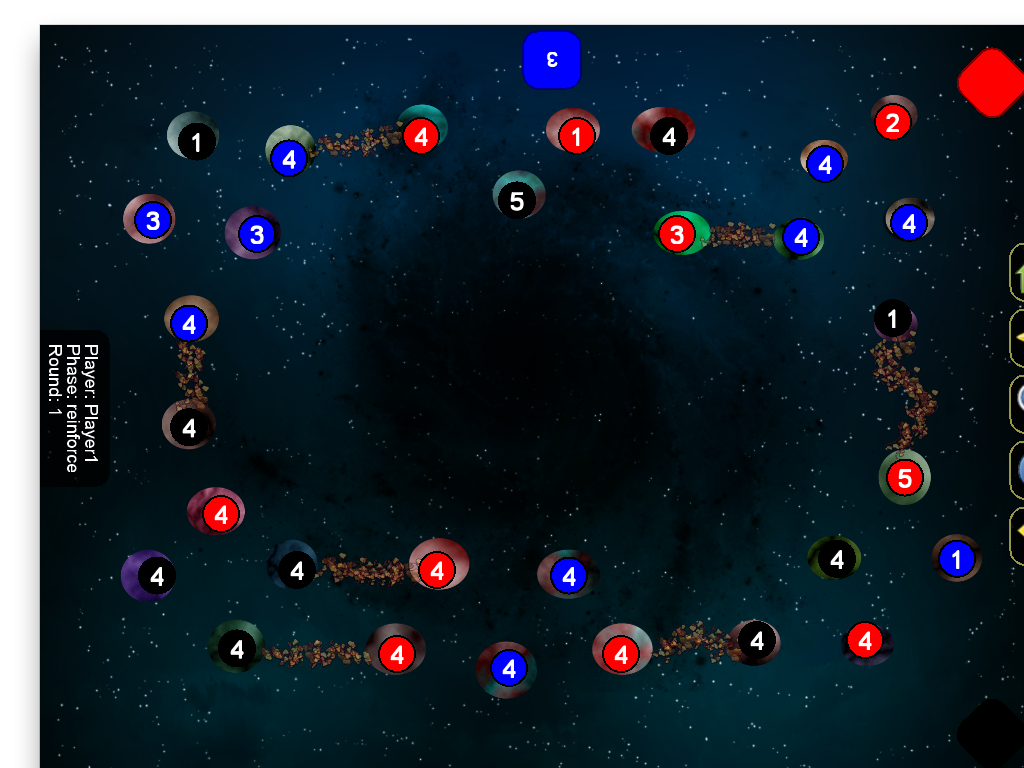
\includegraphics[width=6.5cm]{pic/screenshot04.png}
\caption{Reinforcement.}
\label{fig:reinf}
\end{figure}

The number of troops will be shown in your own menu. The way to place the troops on the map is similar to the one explained for the set up state.

Once you feel ready to go to the next phase click the next phase button. Note that you can not to use all the troops provided, this is made this way because you may want to give some advance to your opponents.

\subsubsection{Using your cards}
You will only be able to use your cards during this phase. For this purpose click on your own menu, then in the cards icon and select the three cards that you want to use. The trade button will be activated if the selected cards are tradable, click it to change the cards for troops.

\begin{figure}[h!]
\centering
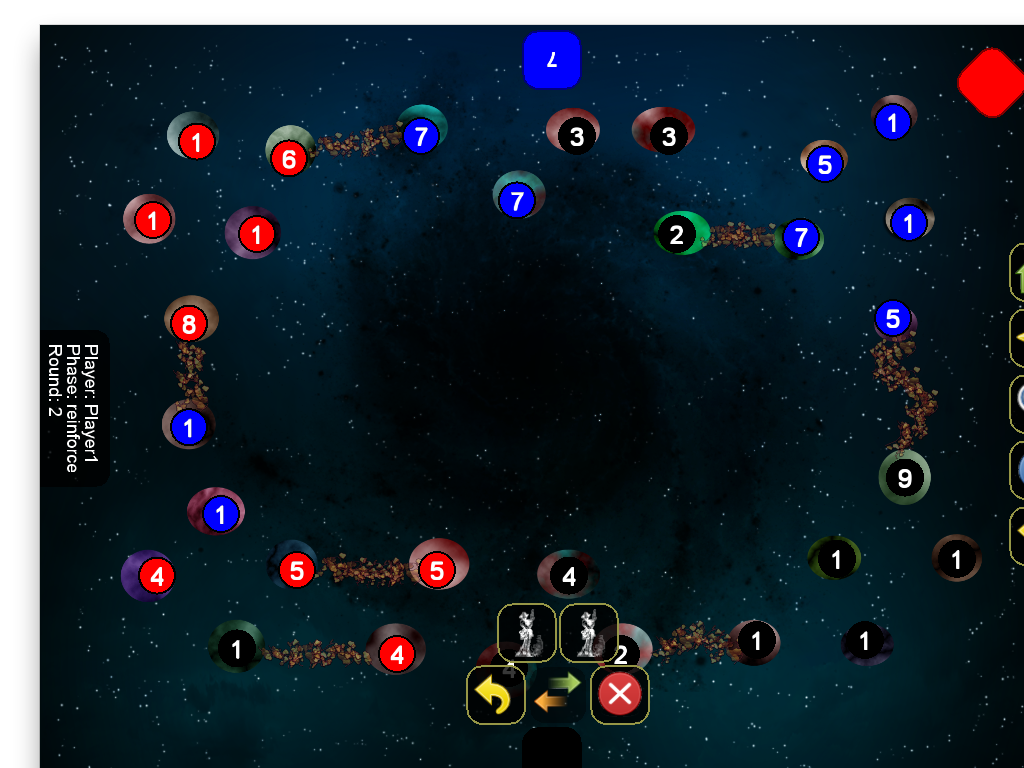
\includegraphics[width=6.5cm]{pic/screenshot05.png}
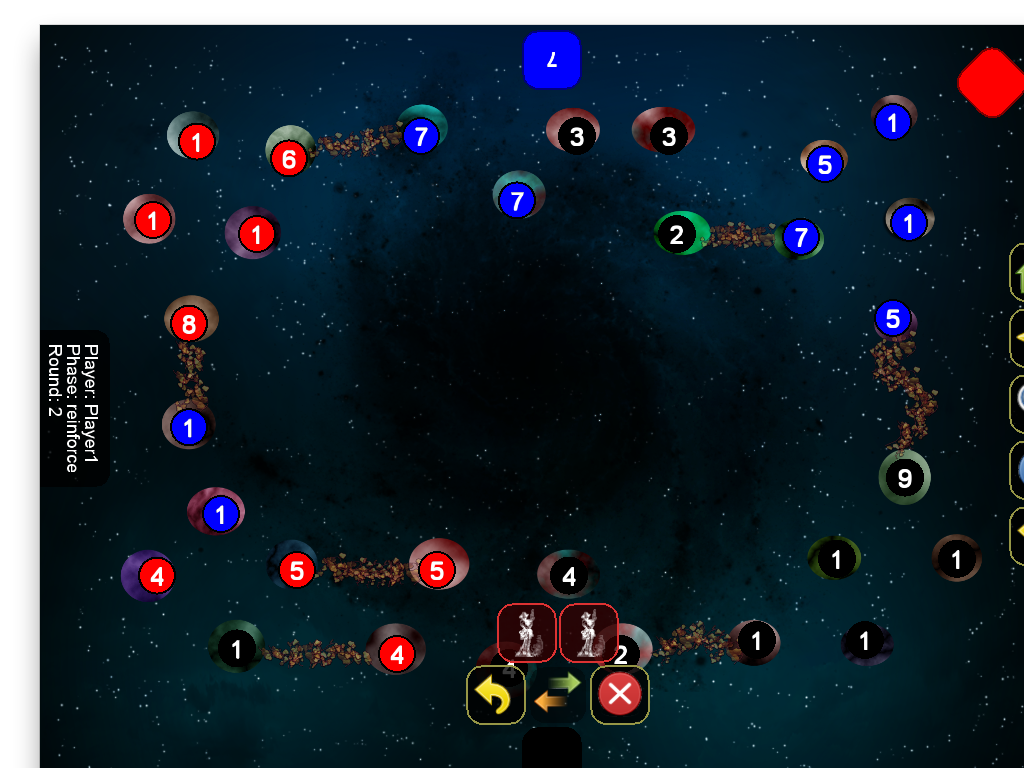
\includegraphics[width=6.5cm]{pic/screenshot06.png}
\caption{Using your cards.}
\label{fig:usecard}
\end{figure}

\subsection{Attack phase}
In the Attack phase your region counters will split, showing two different numbers. The number of the left shows the number of available troops. The number of the right shows the number of used troops. A troop is considered as used when it has attack already another region and has survived.

To attack another region first click on one of your one regions, the neighbor enemy regions will highlight. Now click on the region you want to attack and the combat will start.

\begin{figure}[h!]
\centering
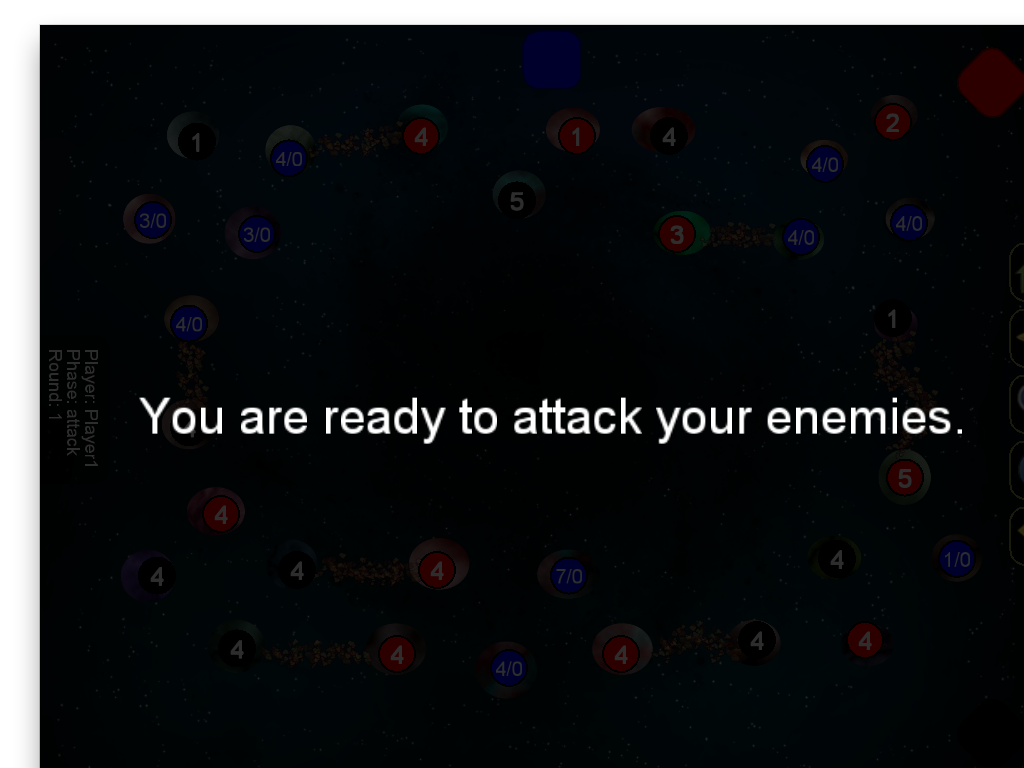
\includegraphics[width=6.5cm]{pic/screenshot07.png}
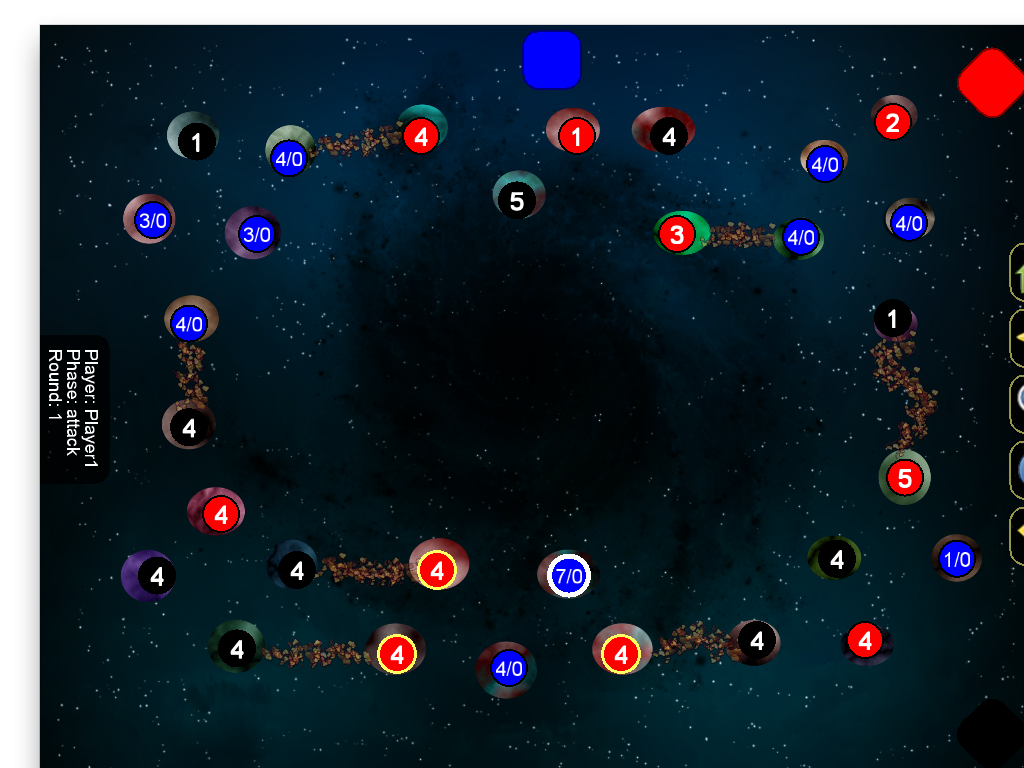
\includegraphics[width=6.5cm]{pic/screenshot08.png}
\caption{Attack phase and highlighted regions.}
\label{fig:attack}
\end{figure}

\subsubsection{Combat}
During the combat both players, attacker and defender, will have to interact:

\begin{itemize}
\item {\bf Attacker}: attacker player will have to select how many troops (from 1 to 3, depending on the number of available troops) he wants to attack with. The number of troops will change by clicking in the {\it sword icons}. Once selected he will have to confirm by clicking on the {\it double sword icon}. Attacker can retreat at any moment by clicking the {\it double arrow icon}.
\item {\bf Defender}: defender player will have to select how many troops (1 or 2, depending on the number of available troops) he wants to defend with. The number of troops will change by clicking in the {\it shield icons}. Once selected, he will have to confirm by clicking on the {\it double sword icon}
\end{itemize}

\begin{figure}[h!]
\centering
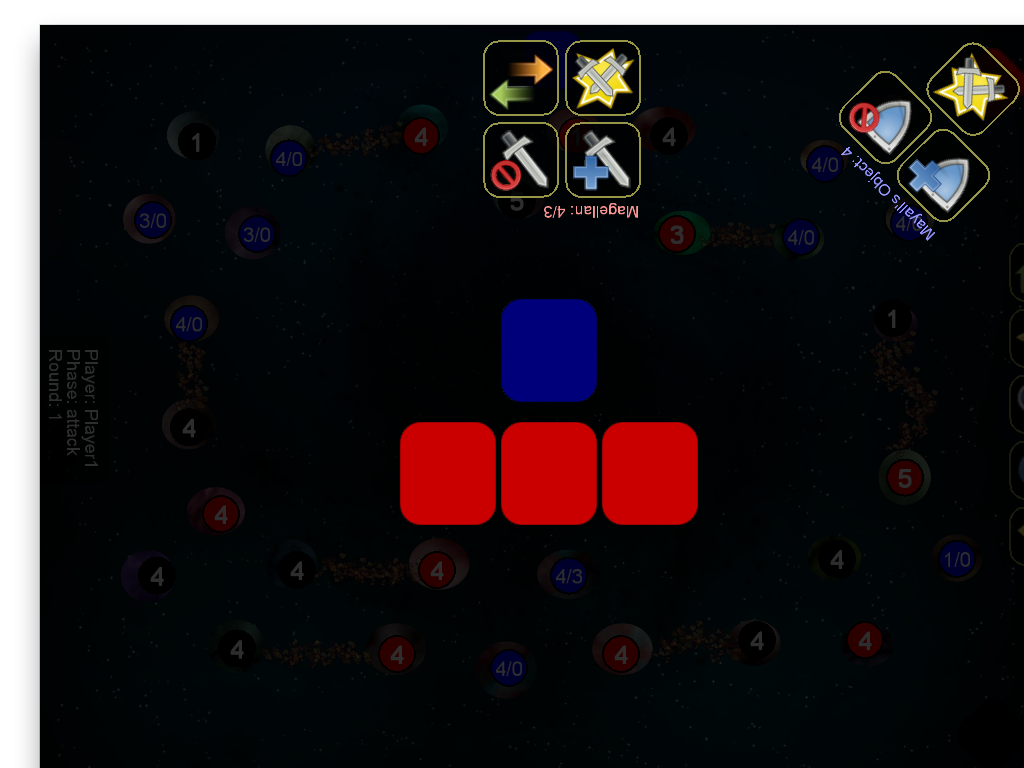
\includegraphics[width=6.5cm]{pic/screenshot09.png}
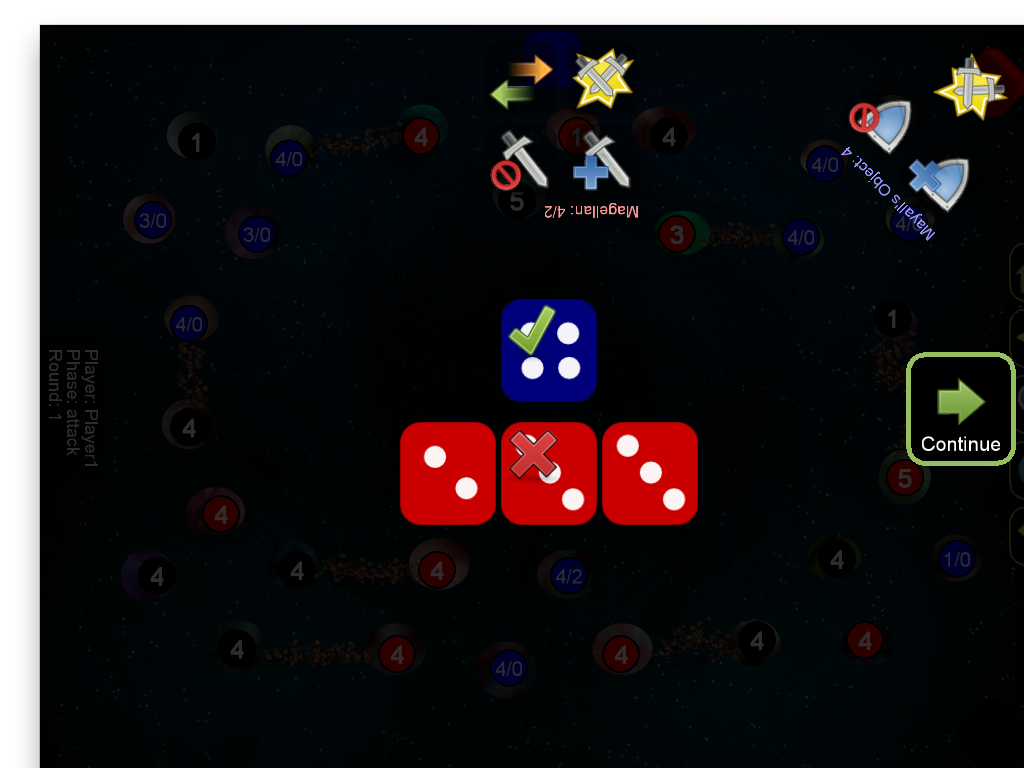
\includegraphics[width=6.5cm]{pic/screenshot10.png}
\caption{Combat before and after throwing dices.}
\label{fig:combat}
\end{figure}

Once both players have confirmed the combat dices will be automatically thrown and checked. Highest dice values from attacker and defender are faced in pairs, the player obtaining the bigger value of each pair will defeat one enemy troop each time.

The combat will automatically end whenever all defending troops are defeated, attacker retreats or all attacker troops are used. If all defending troops are defeated, attacker player will conquer the attacked region and the number of survived units in the last attack will be moved to that region.

\subsection{Movement phase}
In the Movement phase your region counters will also split in the same way as in the Attack phase. In this case a troop is considered as when it has already been moved from one region to another.

To move troops first click the origin region you want to move troops from, the neighbor owned regions will highlight showing where you can move troops to. Once the origin region region is selected, click on it as many times as troops you want to move from that region. Selected troops will be added to player menu counter. Finally, click on any highlighted region to move all selected troops to that region. The moved troops will be showed as used.

\begin{figure}[h!]
\centering
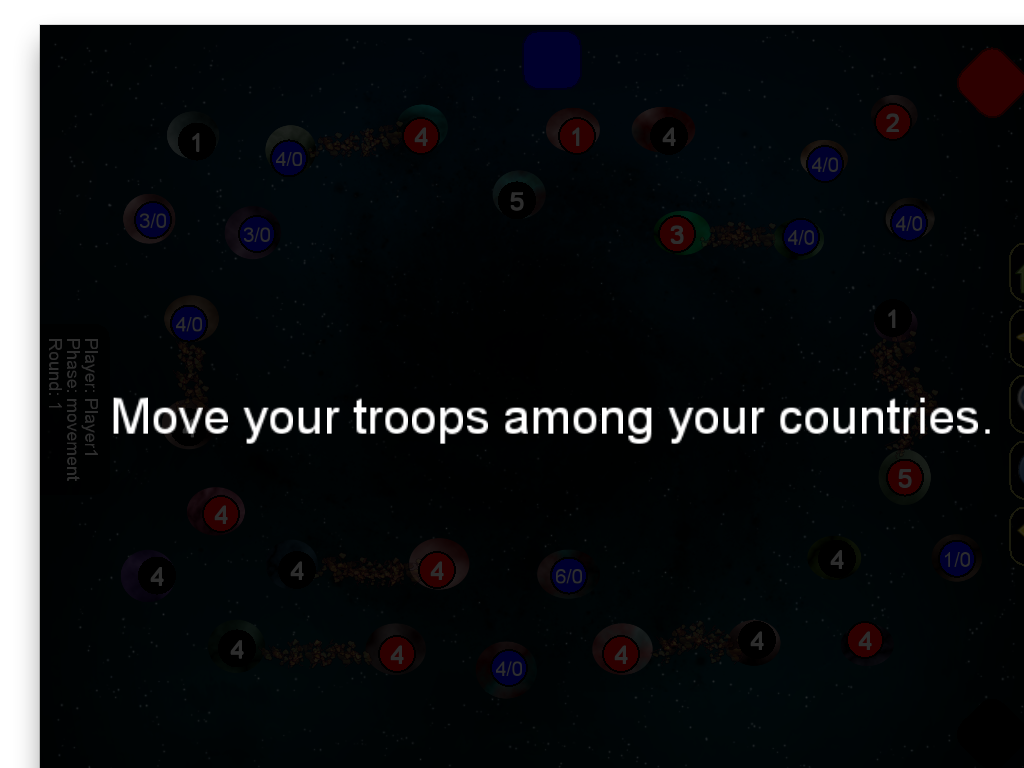
\includegraphics[width=6.5cm]{pic/screenshot11.png}
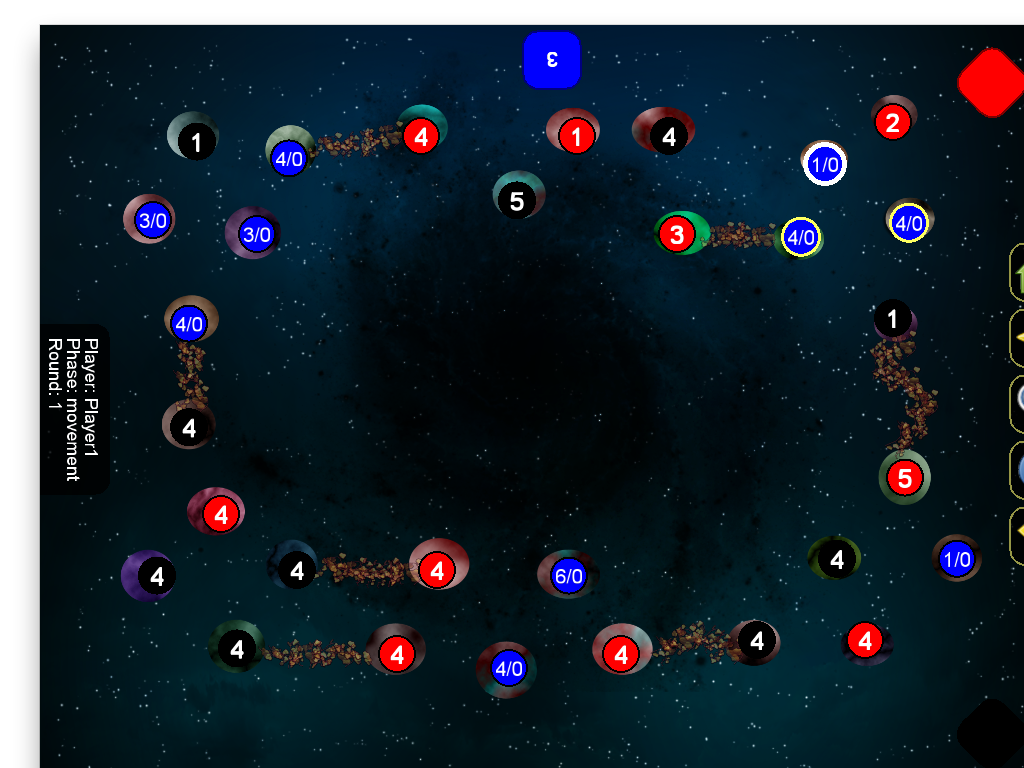
\includegraphics[width=6.5cm]{pic/screenshot12.png}
\caption{Movement phase.}
\label{fig:move}
\end{figure}

\subsection{Winning}
At the end of every turn your mission will be automatically checked. If your mission has been accomplish the game will end.

\section{Main menu}
The main menu will be use to configure the game in the following fields:

\begin{itemize}
\item {\bf Map}: The map can be selected from the top left list.
\item {\bf Profile}: The profile (whole configuration of players) can be selected from the top left list.
\item {\bf Number of players}: The number of players can be selected activating or deactivating each player clicking the small circle on the left of each player.
\item {\bf Player name}: Player name can be changed clicking on it.
\item {\bf Player color}: Player color can be changed clicking on the colored buttons it repetitively.
\item {\bf Player position}: Player position can be changed clicking on the cardinal points buttons. The player position should reflect the real physic player position. N (north) is situated on the top of the actual menu.
\end{itemize}

\begin{todo}[Alberto]
  Add here the new menu options: sound...
\end{todo}

\begin{todo}[Alberto]
  Main menu pic, waiting for last updates
\end{todo}

\section{Player menu}
Player menus will be placed on every player position. Different functionalities are contained in the player menu: next phase, cards, missions and undo.

\begin{figure}[h!]
\centering

\includegraphics[width=1.5cm]{pic/next.png}

\includegraphics[width=1.5cm]{pic/troops.png}

\includegraphics[width=1.5cm]{pic/world.png}

\includegraphics[width=1.5cm]{pic/undo.png}
\caption{Next phase, cards, mission and undo buttons}
\label{fig:playermenu}
\end{figure}

\subsection{Next phase}
Click this button to change phase, attack to movement and movement to next player.

\subsection{Using cards}
Use your cards like described on previous sections (see Figure \ref{fig:usecard}) by opening your personal menu and clicking the cards submenu ({\it shield icon}). Remember to use your hand to hide your cards. Your cards are secret and others player should not know which cards you have.

You will be able to select cards and use them only when a correct combination is selected. Click the central button for this purpose. Select cards and discard them clicking the right button ({\it red circle}). Go back clicking the left button. 

\subsection{Checking missions}
Open your personal menu and click the mission button ({\it world globe icon}) to display your mission. Remember to use your hand to hide your mission, it is secret and other players should not know it. Click on the mission text to go back to the previous menu.

\begin{figure}[h!]
\centering
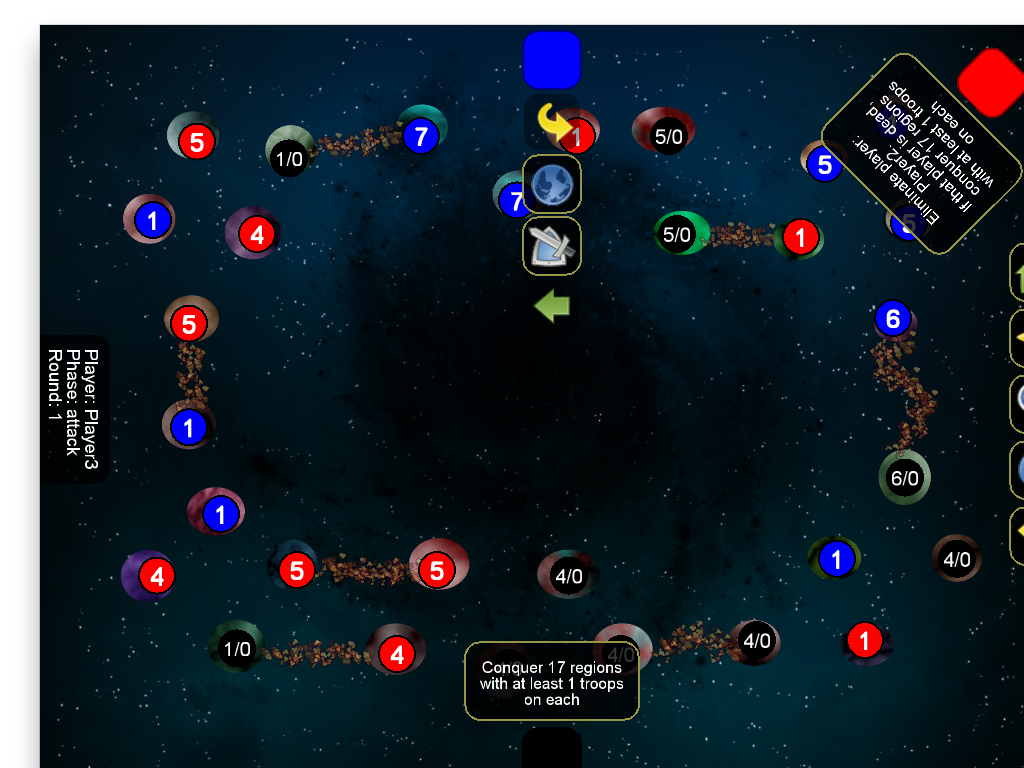
\includegraphics[width=10cm]{pic/screenshot13.png}
\caption{Checking missions.}
\label{fig:checkmis}
\end{figure}

\subsection{Undo action}
\begin{todo}[Alberto]
Will this be done?
\end{todo}

\section{Game menu}
The game menu will provide you some tools to use during the game play. It will be displayed vertically on the right side of the screen. The options, described deeply below, are, from top to bottom: open option menu, move map, zoom map, rotate map and restore.

\begin{figure}[h!]
\centering

\includegraphics[width=1.5cm]{pic/home.png}

\includegraphics[width=1.5cm]{pic/move.png}

\includegraphics[width=1.5cm]{pic/zoom.png}

\includegraphics[width=1.5cm]{pic/rotate.png}

\includegraphics[width=1.5cm]{pic/undo.png}
\caption{Option menu, move, zoom, rotate and restore icons}
\label{fig:mapmenu}
\end{figure}

\subsection{Options menu}
Click the option menu button ({\it green house icon}) to display a floating menu with the following options from left to right: close, save, help and quit.

\begin{itemize}
\item {\bf Close}: close the floating menu and return to the game.
\item {\bf Save}: save the game in the actual state.
\item {\bf Help}: display help
\item {\bf Quit}: end game and go to main menu.
\end{itemize}

\begin{figure}[h!]
\centering
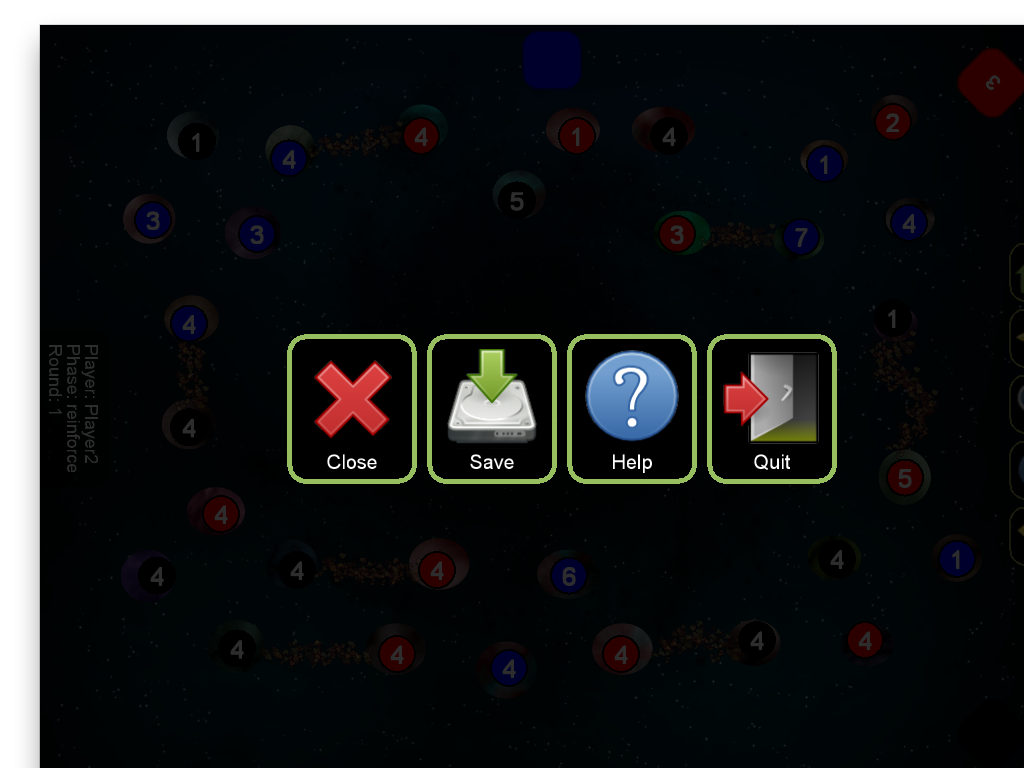
\includegraphics[width=10cm]{pic/screenshot14.png}
\caption{Options menu}
\label{fig:optionmenu}
\end{figure}


\subsection{Moving}
Use this option to move the map. Click the moving button ({\it compass icon}) and then click and drag on the map to rotate.

\subsection{Zooming}
Use this option to zoom in or out the map. Click the zoom button ({\it magnifier icon}) and then click and drag up to zoom in and down to zoom out.

\subsection{Rotating}
Use this option to rotate the map. Click the rotate button ({\it blue twisted arrow}) and then click and drag up to rotate counterclockwise and down to rotate the map clockwise.

\subsection{Restoring}
Use this button to restore the initial visual settings of the map. Click the restore button ({\it yellow twisted arrow}) and the configuration will be restored automatically.

\section{Customization}
We provide you some additional options to make the game experience more complete. Do you maybe want to play another map? Create a new one! Do you always play with the same group of friends? Create a profile!

\subsection{Map}
Maps can be created and added to the game by following a simple set of rules. Read our {\it Map manual} for further information.

\subsection{Profile}
Profiles can be easily saved and loaded on the main menu. 

\begin{todo}[Alberto]
  This is shitty, correct it xD
\end{todo}


\end{document}